Der SUS-Fragebogen wurde den Probanden unter den gleichen Anforderungen vorgelegt 
(Bezug nur auf das Verfahren bei der Authentisierung und die TOTP-App).
In Abb. \ref{fig: studie ergebnisse auth sus boxplot} sowie Tab. \ref{tab: studie 
ergebnisse auth sus boxplot} werden Blue TOTP und das traditionelle TOTP-Verfahren 
gegenübergestellt.
\begin{figure}
    \centering
    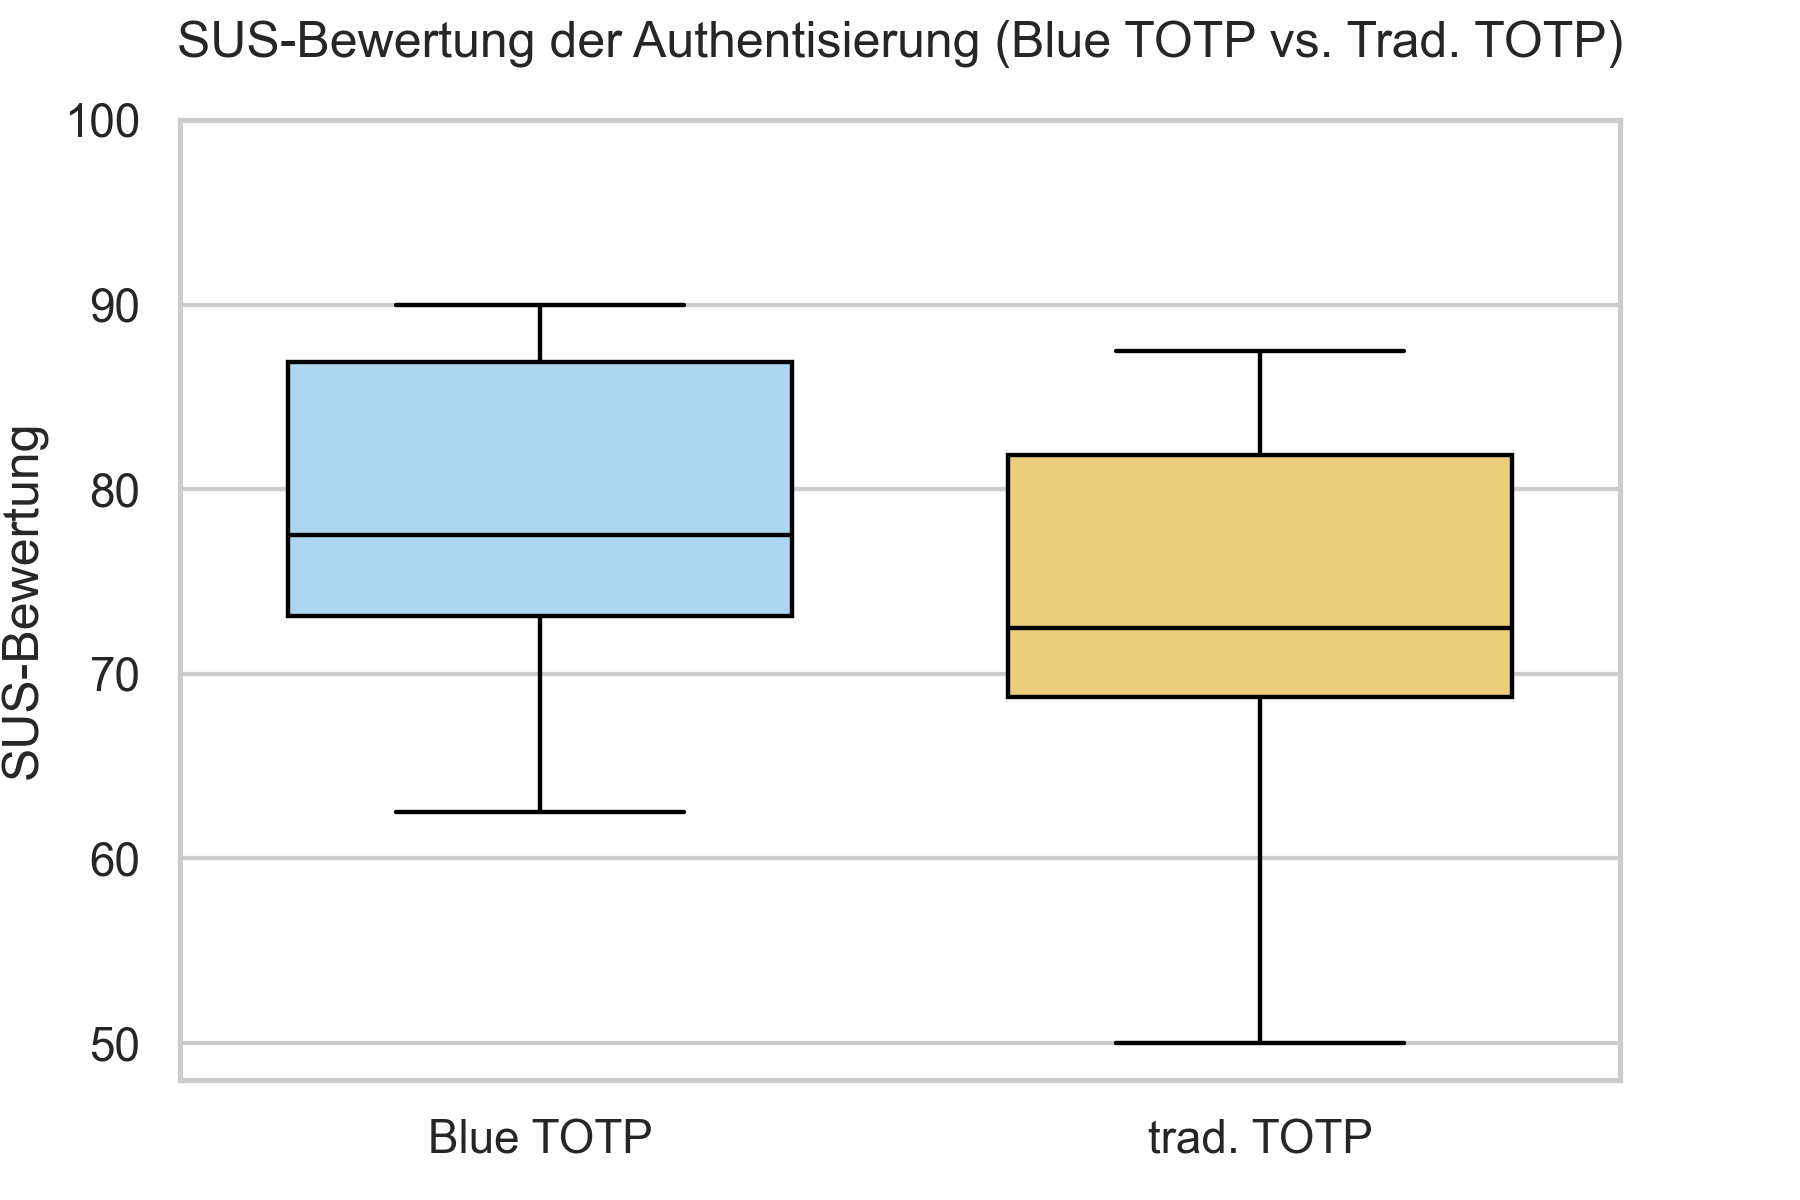
\includegraphics[width=0.6\linewidth]{data_processing/questionaires/results/usage_sus_boxplot.png}
    \caption[SUS-Bewertung der Authentisierung (Blue TOTP vs. trad. TOTP)]{SUS-Bewertung der Authentisierung (Blue TOTP vs. trad. TOTP)}
    \label{fig: studie ergebnisse auth sus boxplot}
\end{figure}
\begin{table}
    \begin{center}
    \begin{tabular}{| l | c | c | c | c |}
        \hline
        \textbf{Verfahren} & \textbf{Q1} & \textbf{Median} & \textbf{Mittelwert} & \textbf{Q3}  \\
        \hline
        Blue TOTP & 73 & 78 & 79 & 87 \\
        \hline
        Trad. TOTP & 69 & 73 & 73 & 82 \\ 
        \hline
    \end{tabular}
    \end{center}
    \caption[SUS-Bewertung der Authentisierung (Blue TOTP vs. Trad. TOTP)]{SUS-Bewertung der Authentisierung (Blue TOTP vs. Trad. TOTP)}
    \label{tab: studie ergebnisse auth sus boxplot}
\end{table}
Das Boxplot deutet darauf hin, dass die Verteilung der SUS-Bewertungen beider 
Verfahren im Interquartilbereich sich ähneln und nur auf der Y-Achse verschoben sind. 
Es ist deutlich erkennbar, dass das traditionelle in allen Werten Blue TOTP 
nachsteht. Die Normalverteilung der Differenzen der SUS-Berwertungen pro Proband wurde mit dem Shapiro-Wilk-Test bestätigt ($p=0{,}4439$) und daher ein Paired t-Test für die SUS-Bewertungen durchgeführt. Allerdings konnte keine statistische Signifikanz zwischen den beiden SUS-Bewertungen festgestellt werden ($p=0{,}2366$, $\alpha = 0{,}05$). Blue TOTP erzielt einen Median von 78 Punkten und das traditionelle 
Verfahren nur 73 Punkte. Dieser Abstand von ca. 5 Punkten lässt sich auch bei den 
anderen Größen 1. Quartil, Mittelwert und 3. Quartil beobachten, die zwischen 4 bis 6 
Punkten auseinander liegen (vergl. Tab. \ref{tab: studie ergebnisse auth sus 
boxplot}). Folgt man den Erkenntnissen von \textcite{Sauro}, so liegt dieser Bereich 
im annähernd linearen Verlauf der S-Kurve, die den prozentualen Wert einer 
SUS-Punktzahl wiedergibt. Demnach wäre der eben beschriebene  Unterschied von ca. 5 
Punkten linear zum prozentualen Wert (nicht im Verhältnis 1:1).
\\\\
Auch diesmal haben die Probanden am Ende des Fragebogens die empfundene 
Nutzerfreundlichkeit angegeben. Die SUS-Bewertungen und entsprechenden 
SUS-Punktzahlen zu der empfundenen Nutzerfreundlichkeit sind in Abb. \ref{fig: studie 
ergebnisse auth sus vs 11} dargestellt.
\begin{figure}
    \centering
    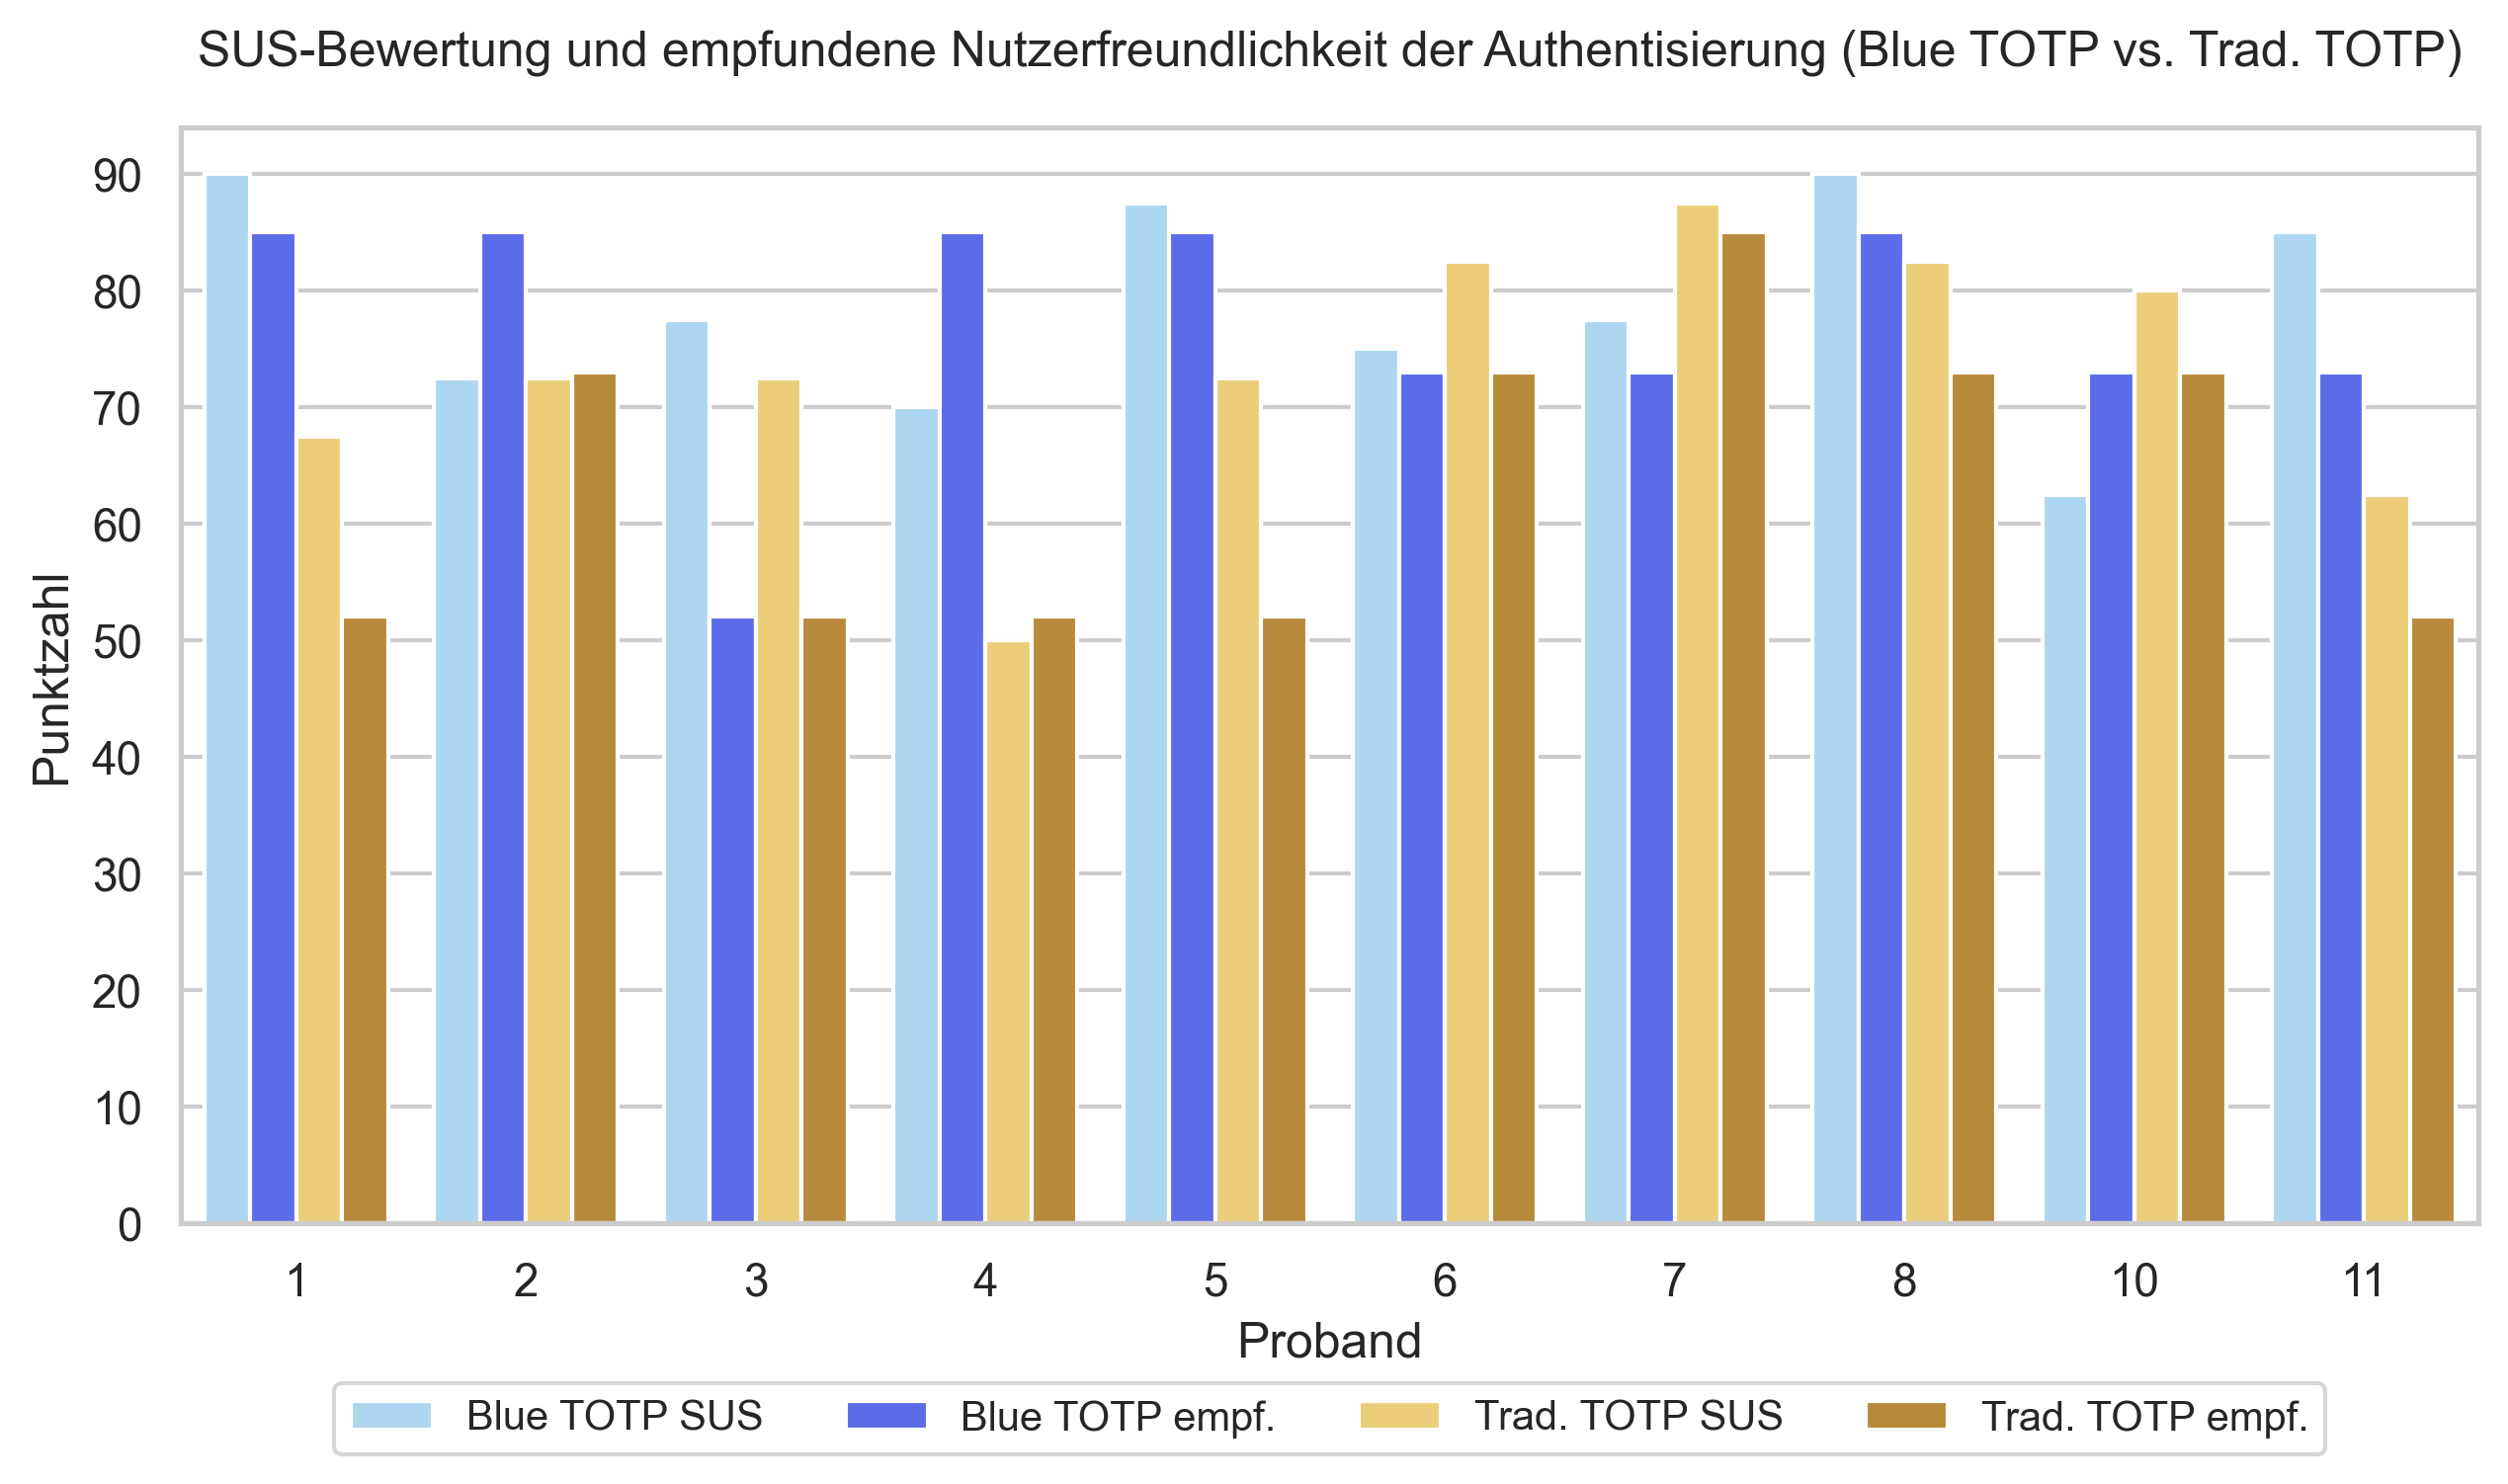
\includegraphics[width=0.8\linewidth]{data_processing/questionaires/results/usage_sus_vs_sus11.png}
    \caption[SUS-Bewertung und empfundene Nutzerfreundlichkeit (Authentisierung)]{SUS-Bewertung und empfundene Nutzerfreundlichkeit der Authentisierung (Blue TOTP vs. trad. TOTP)}
    \label{fig: studie ergebnisse auth sus vs 11}
\end{figure}
Bzgl. Blue TOTP sind zwei starke Differenzen erkennbar bei P3 (26 Punkte) und P4 (15 
Punkte). Dagegen gibt es bzgl. des traditionellen Verfahrens drei starke Differenzen 
bei P3 und P5 mit je 21 Punkten sowie bei P1 mit 16 Punkten. Bildet man den 
Mittelwert der Differenzen getrennt für beide Verfahren, erhält man für Blue TOTP 
$\bar{x}_{Diff} = 9{,}5$ mit einer Standardabweichung von $\sigma_{Diff} = 7,3$. Für 
das traditionelle Verfahren erhält man $\bar{x}_{Diff} = 9{,}8$ und eine 
Standardabweichung von $\sigma_{Diff} = 7{,}2$. Das heißt, für beide Verfahren 
verhalten sich die Differenzen zwischen der tatsächlichen SUS-Punktzahl und der 
\glqq empfundenen\grqq{} SUS-Punktzahl gleichermaßen. Die empfundene Punktzahl 
bestätigt die tatsächliche Punktezahl weitestgehend.
\\\\
Die Aussagen des SUS werden mit einer $5$-stufigen Skala bewertet. Gibt man jeder 
dieser Stufen entsprechend die Werte $0$ bis $4$ ($0$ vollständige Ablehnung der 
Aussage, $2$ neutral, $4$ vollständige Zustimmung) und invertiert dann die negativ 
formulierten Aussagen, kann für jede Aussage Mittelwerte bilden. Diese sind für beide 
Verfahren in Tab. \ref{tab: studie ergebnisse auth sus vs 11 single means} 
dargestellt. Das heißt Werte $> 2$ sind positiv behaftet und Werte $< 2$ negativ.
\begin{table}
    \centering
    \begin{center}
    \begin{tabular}{| l | c | c | c | c | c | c | c | c | c | c |}
        \hline
        \textbf{Aussage} & 1 & 2 & 3 & 4 & 5 & 6 & 7 & 8 & 9 & 10 \\
        \hline
        \textbf{Mittelwert Blue TOTP} & $3{,}1$ & $3{,}0$ & $3{,}6$ & $3{,}1$ & $3{,}1$ & $2{,}9$ & $3{,}6$ & $2{,}9$ & $2{,}8$ & $3{,}4$ \\  
        \hline
        \textbf{Mittelwert Trad. TOTP} & $2{,}5$ & $2{,}7$ & $2{,}9$ & $3{,}5$ & $2{,}9$ & $2{,}7$ & $3{,}2$ & $2{,}9$ & $2{,}8$ & $3{,}1$ \\
        \hline
    \end{tabular}
    \end{center}
    \caption[Durchschnittliche Bewertung pro Aussage des SUS (Authentisierung)]{Durchschnittliche Bewertung pro Aussage des SUS (Authentisierung Blue TOTP vs. Trad. TOTP)}
    \label{tab: studie ergebnisse auth sus vs 11 single means}
\end{table}
Interessant sind dabei die Mittelwerte zu den Aussagen 1, 3, 4 und 8. Bei den 
Aussagen 1 (regelmäßige Nutzung des Systems) und 3 (Nutzung des Systems einfach) 
herrscht eine starke Differenz von $0{,}6$ bzw. $0{,}7$ zu Gunsten von Blue TOTP. Bei 
Aussage 4 (Hilfe einer technisch versierten Person nötig) steht das traditionelle 
Verfahren mit $\bar{x} = 3{,}5$ über Blue TOTP $\bar{x} = 3{,}1$. Zuletzt sei noch 
Aussage 8 erwähnt, die das System als umständlich zu nutzen beschreibt. Hier sind 
beide Verfahren mit $\bar{x} = 2{,}9$ gleich auf.